\documentclass[../main.tex]{report}
	
\begin{document}
    \label{sec:odd_prob}
\subsubsection{Ensembles probabilistes impairs}
Bien que ces ensembles aléatoires suivent la distribution de $\pi(x)$, il manque une propriété importante des nombres premiers: à l'exception de $2$, tous les nombres premiers sont impairs.

Nous allons alors modifier l'algorithme mentionné précedemment afin de générer des ensembles ayant cette propriété. 
Soit $O_n := E_n \cap 2 \mathbb{N} +1$ l'ensemble des entiers impairs inférieurs ou égaux à $n$. 
Soit alors l'ensemble aléatoire 
$U_{k_n} \subset \{O_n \cup \{2\}\}$
tel que $\forall~i \in \{O_n \cup \{2\}\}$, le probabililité que $i$ soit dans l'ensemble $U_{k_n}$ soit:

\[
P(i \in U_{k_n}) = 
\left\{ 
    \begin{array}{cl}
         0 & \mbox{si}~i = 1 \\
         1 & \mbox{si}~ 2 \leq i < 9 \\
         \frac{2}{\log n} & \mbox{si}~i \geq 9
    \end{array}
\right.
\]

Le fait que $P(i \in U_{k_n}) = 1$ pour les entiers impairs inferieurs à 9 découle du fait que $2/\log(n) > 1$ pour ces entiers.

On observe alors que ces suites débutent avec les mêmes éléments: $ (2,3,5,7,...) $, mais contiennent des éléments aléatoires à partir du 5\up{e} terme. 
Pour tout $n \geq 5$, la fonction $\sigma$ est une valeur aléatoire d'espérance: 
\[
E[\sigma(n)] = 
4 + \sum_{i=5}^{\lfloor{n/2}\rfloor} \frac{2}{\log (2i-1)}
\]

En réécrivant l'équation \ref{eq:SommeDeRiemann} de la page \pageref{eq:SommeDeRiemann} en une somme de Riemann de pas constant = 2, on obtient que:
\[
S\left(\frac{1}{\log(x)}\right) = \sum_{k=0}^{n}\frac{2}{\log 2+k}
\]


\begin{figure}[H]
\centering
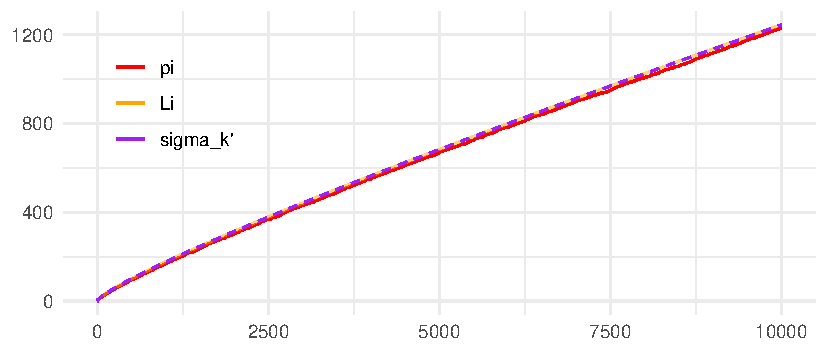
\includegraphics[width=\textwidth,height=6cm]{comparison_odd_prob}
\caption{Graphes des fonctions $\pi$ et $\sigma$.}
\label{fig:comparison_sigma_prob}
\end{figure}

\begin{figure}[H]
	\centering
	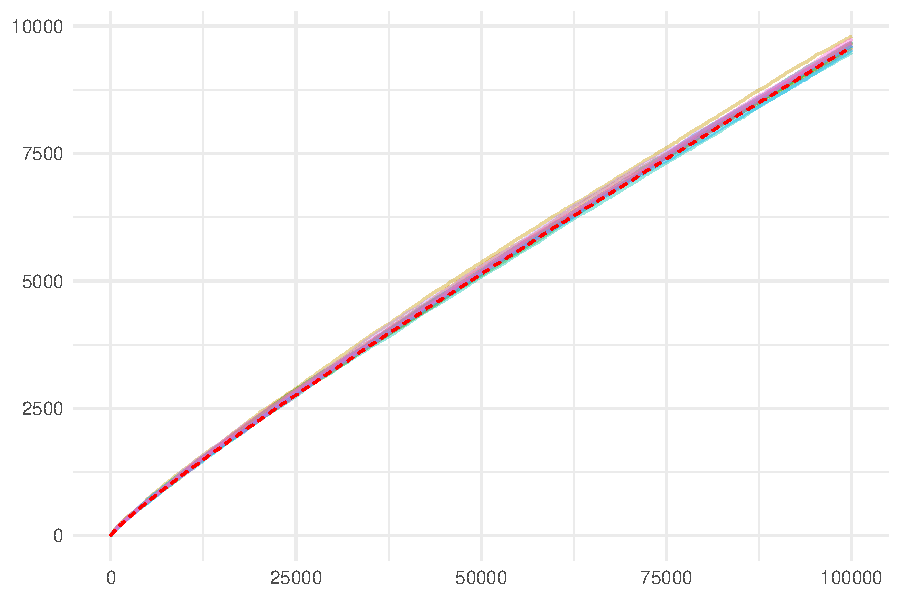
\includegraphics[width=\textwidth]{prob_sample_odd}
	\caption{graphes des fonctions $\sigma_k$ pour $k \leq 25$ (25 premiers ensembles impairs) et $\pi$}
	\label{fig:prob_sample_odd}
\end{figure}

\end{document}